\section{Application of the \cof Protocol without Checkpoints\label{section:application}}

The \cof protocol circumvents one of the major limitations of current
MPI implementations: the lack of confidence that the MPI library is capable of
successfully completing communications once a failure happened. As illustrated
above, forward recovery strategies are
capable of taking advantage of this technique and provide efficient fault
tolerance support that does not require periodic checkpointing.
However, when a failure strike, the \cof protocol still incurs 
checkpoint I/O overhead. 
In this section, we explain how the \cof protocol can be efficiently integrated
with already resilient, non-MPI applications to completely eliminate 
all checkpointing activity. We will illustrate the approach with a 
fault-tolerant database management system, SciDB.

Fault tolerant database management exposes a set of requirements that is best
addressed today using replication and transactional operations.
% , for which the \cof protocol will provide little improvement.
SciDB~\cite{scidbwhitepaper} combines database operations and many scientific
specific operations (including linear algebra routines) to create a highly
expressive request query language suitable for scientists to solve their data
analysis problems. The SciDB system is not implemented on top of MPI, 
mainly because of the lack of fault tolerance capabilities from
the MPI Standard. It makes use, however, of the MPI based
distributed linear algebra operations in ScaLAPACK, to provide, among other
things, various factorization routines. Because most MPI implementations are not
usable after a process failure, and high availability is a necessity in database
management systems, the SciDB implementation cannot integrate the MPI library in
its main process. As a result, the linear algebra operations are called 
from separate processes: a query coordinator orders the distributed database
managers to locate the data on which the factorization operation must be
applied and to expose this data in the expected ScaLAPACK layout using one
shared memory segment per node; it then launches a ScaLAPACK/MPI application
that attaches to this memory segment and applies the operation on it. If a
failure hits a node, the MPI application aborts, and the {\it mpirun} child
process reports the error to the data query coordinator. The original data is
recovered from the database management system (using database-specific fault
tolerant techniques), and the linear algebra operation is relaunched from scratch
on the original data.


\begin{figure}
\begin{center}
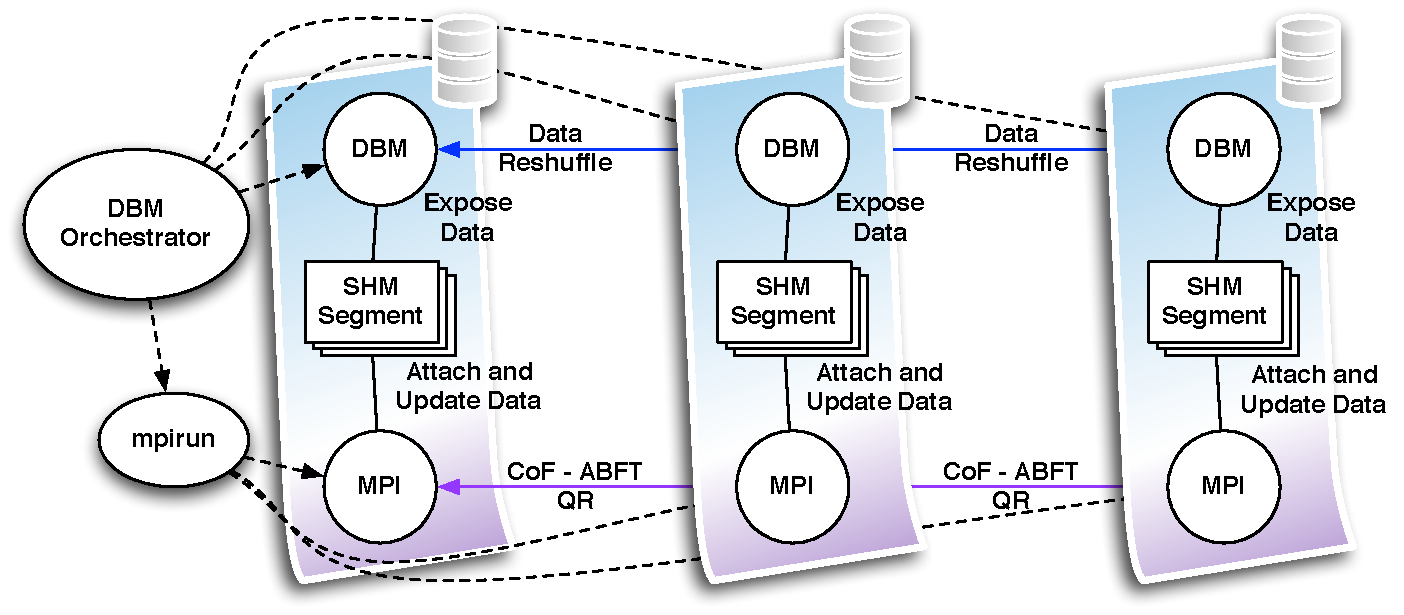
\includegraphics[width=.9\linewidth]{figures/CoF-DDB.pdf}
\caption{SciDB / CoF ABFT ScaLAPACK Integration\label{fig:scidb-cof}}
\end{center}
\end{figure}


This approach can be improved using the \cof protocol and an ABFT
implementation of the factorization operation. The idea is depicted in
Figure~\ref{fig:scidb-cof}. SciDB and ScaLAPACK are coupled in a similar
way; however, the DB managers compute the initial checksum of the
original data, and expose both the data and checksum to the
ABFT-ScaLAPACK process. The ABFT operation is applied, and if no failure
happens, the result of the factorization is accessible in the shared
memory segments (the checksum data can then be discarded by the DB
managers). If a failure occurs, the MPI process updates the shared
memory segments with the meta information of the checkpoint (values of
the loop counters, etc...); the content of the shared memory segments is
analog to the checkpoints performed in the normal \cof protocol. Then,
the MPI processes quit and the {\it mpirun} child process reports the
error to the database coordinator. Instead of fixing the data issue at
the DB level, the coordinator immediately relaunches a new
ABFT-ScaLAPACK operation on the same set of nodes plus a spare node with
an empty shared memory segment, the ABFT algorithm recovers the data and
the original operation resumes. Upon successful completion, the
{\it mpirun} child process reports to the database coordinator
that the result is in the shared memory segments.

This approach is advantageous compared to both the original design and
the checkpoint-based \cof approach. 
%
  Instead of restarting from scratch after each failure, the
  factorization incurs only the small recovery overhead of ABFT, ensuring a
  faster time-to-solution for the linear algebra operation. In exchange, a small
  overhead, for creating and maintaining the checksum data during the operation,
  is imposed on the failure-free case.
%
Second, this approach removes the cost of writing the checkpoint to a
  file: the shared memory segment that survives the exit of the MPI processes
  where the node was not subject to a failure and the checksum information
  maintained by the ABFT algorithm are sufficient to recover the missing
  data. The segment of memory on which the operation is computed is made
  remanent, creating the bulk of the checkpoint data and reducing to an
  insignificant value the cost of checkpointing when a failure occurs. This will
  be demonstrated in the experimental section, below.

 
